\chapter{Configuration de \textit{Microsoft Azure}}\\

\section{Mise en place pour 1 station}\\

Vous allez abandonner notre \textit{RaspberryPi} pendant quelques instant pour se focaliser sur la création d'une instance dans le \textit{Cloud} pour que vous puissiez envoyer les données.\\

Pour réaliser cette partie, munissez vous de vos identifiant \textit{Microsoft Azure}.\\

\subsection{Explication des fonctionnalités proposées par \textit{Microsoft}}
Avant de commencer, nous allons détailler un peu plus précisément le cheminement que vont avoir nos données. Comme souvent une image vaut mieux qu'un long discours, je vous laisse observer : 
%dessin ici photoshop Hub -> Time Serie Insight

%description de l'image a faire ici

Nous allons expliciter deux méthodes différentes de gestion de \textit{Azure} pour vous montrer le champs des possible. En effet, vous pouvez utiliser le portail qui nous est proposé par \textit{Microsoft} ou bien utiliser ce qui s'appelle \textit{L'Azure CLI} pour \textit{Azure Command Line Interface}.

\subsection{Création d'un Hub d'évènements sur \textit{Azure} avec la \textit{CLI}}\\

\subsubsection{Installation de l'Interface en Ligne de Commande de \textit{Azure}}\\

Pour cette partie il n'est donc pas nécessaire de se rendre sur le portail. Mais avant toute chose, vous devez installer l'interface en ligne de commandes \textit{d'Azure}.\\

\begin{enumerate}
	\item Installer \href{https://nodejs.org/download/release/latest/}{\textit{Node.js}} en choisissant l'extension \textit{.msi} pour x64 ou x32 selon si votre système est en 64bit ou 32bit.
	\item Lancer un terminal \textit{git bash}.
	\item Tapez les deux commandes suivantes pour vérifier que \textit{Node.js}  et \textit{NPM} (Node Package Manager) a bien été installé. \textit{NPM} est l'utilitaire qui va nous permettre d'installer \textit{Azure}
	\begin{lstlisting}[style=MyBashStyle]
	node -v
	npm -v
	\end{lstlisting}\\
	Vous devriez avoir ce résultat : %photo ici
	\item Ensuite entrer la commande :
	\begin{lstlisting}[style=MyBashStyle]
	npm install -g azure-cli
	\end{lstlisting}\\
\end{enumerate}\\
Et voilà, Azure est installé, vous devriez pouvoir le lancer en tapant \textit{azure} dans votre terminal \textit{git bash}. Voici ce que vous devriez obtenir : %photo ici

\subsubsection{Création d'un groupe de ressources et d'un Hub d'évènement}\\

Maintenant, il va falloir créer nos instance qui vont récupérer les valeurs envoyée par notre station.

\begin{enumerate}
	\item Connecter vous avec votre compte \textit{Azure} :
	\begin{lstlisting}[style=MyBashStyle]
	azure login
	\end{lstlisting}\\
	Aller alors sur la page : \href{https://aka.ms/devicelog}{https://aka.ms/devicelog} pour entrer le code qui vous sera spécifié sur votre terminal. Entrer ensuite vos identifiants. Vous devriez alors être connecté. %photo ici
	\item Taper la commande :
	\begin{lstlisting}[style=MyBashStyle]
	azure group list
	\end{lstlisting}\\
Vous verrez alors la liste des groupes de ressources déjà existant. Vous allez alors créer un groupe de ressources par la commande : 
	\textbf{NOTE : POUR LE DOSSIER, LE GROUPE A POUR NOM \textit{IoT}. VOUS POUVEZ RENSEIGNER LE NOM QUE VOUS SOUHAITEZ}\\
	\begin{lstlisting}[style=MyBashStyle]
	azure group create IoT westeurope
	\end{lstlisting}\\
westeurope détermine le serveur où le groupe sera créé. %photo ici
\\
Si vous refaites la commande de l'étape N°2, vous devriez voir apparaitre votre nouveau groupe fraichement créé sur la liste.
	\item Maintenant, vous allez devoir télécharger le code de la station, comme vous l'avez fait pour la \textit{RaspberryPi} dans le chapitre 2. En effet, il y a un fichier qui sert de patron pour les paramètres à appliquer pour la commande qui suivra. Ainsi, entrer les commandes : 
	\begin{lstlisting}[style=MyBashStyle]
	cd
	git clone XXXXXXXXXXXXXXXXXXXXXXXXXXXXXXXXXXXXXXXXXXX
	\end{lstlisting}\\
	\item Maintenant, vous pouvez faire la commande :
	\begin{lstlisting}[style=MyBashStyle]
azure group deployment create -g IoT -n deployment1 -f ~/stage_drancy/IoT.json
	\end{lstlisting}\\ %PATH a changer

Vous allez être inviter à entrer différentes informations. Les informations que vous allez rentrer seront indispensable car devront être ajouté au code de la station pour pouvoir envoyer les données. Les valeurs sont des chaines de caractère, celle mise en photo sont arbitraires pour le dossier, veuillez entrer une valeur différente.
	\begin{enumerate}
	\label{CLI}
		\item namespaceName : Il est conseillé de rajouter NS à la fin pour vous y retrouver ensuite. %photo ici
		\item eventHubName : Il s'agit de l'instance à proprement parlé qui va recevoir les données. vous pouvez par exemple entrer une valeur du type "Station".
		\item consumerGroupName : Pour celle valeur, je vous conseille d'entrer la même que pour namespaceName mais de remplacer NS par GN.
	\end{enumerate}\\ 
Le déploiement peut prendre un peu de temps. Si cela ne fonctionne pas, retenter en entrant des nom différents.
Une fois le déploiement terminé. Plusieurs valeurs sont à noté et sauvegarder précieusement.

\textbf{Notez d'une part la valeur des trois champs que vous avez indiquer !.
De plus, il vous faut noter la valeur de \textit{SharedAccessKeyName} et \textit{SharedAccessKey}}

\end{enumerate}

Nous en avons terminé avec la création de l'instance qui va récupérer les données envoyé par la station. Il faut maintenant vous occuper de l'instance qui va traiter les données reçu.

\subsection{Création d'un portail \textit{Time Series Insights}}

\textit{Microsoft} à pensé à nous puisque il a crée un module qui s'occupe seul de traiter les données d'une source pour ensuite créer des courbes et ainsi voir le suivi dans le temps. Sans cela, le processus aurait été nettement plus long puisqu'il aurait fallut d'une part stocké ces valeurs pour ensuite les traiter et devoir créer une interface qui puisse afficher les valeurs.

Vous allez pour cette partie nous rendre sur le \href{https://portal.azure.com}{\textit{Portail Azure}}. Nous allons dans un premier temps jeter un coup d'oeil sur le groupe que vous avez créé dans la partie d'avant. %photo ici 
\\

Cliquer à gauche sur \textit{Groupes de ressources}. Vous devriez voir apparaitre un Hub D'évènement qui porte le nom de votre \textit{namespaceName} de la partie précédente. Maintenant si vous cliquez sur ce Hub d'évènement, en bas de la vue d'ensemble devrait apparaitre un Hub d'évènement dont le nom est celui que vous avez entré pour le champs eventHubName précédemment. Une fois n'est pas coutume, continuons notre jeux des poupées russes et cliquer dessus. Une fois encore, vous devriez voir apparaitre en bas deux groupe de consommateur. Le premier, \textit{Default} est.... celui utilisé par défaut si jamais vous ne voulez pas créer de groupe de consommateur. Mais c'est toujours mieux d'en avoir un dont on connait le nom par soucis de visibilité. Le second est celui que vous avez créé tout à l'heure.\\

Maintenant que vous êtes rassuré sur les lignes de commande de la partie précédente nous allons pouvoir créer notre instance de traitement des données.\\
\begin{enumerate}
	\item Cliquer sur le \textit{+} en haut à gauche de votre portail.
	\item Dans la barre de recherche du menu qui vient de s'ouvrir, entrer \textit{"Time Series"}
	\item Choisissez alors \textit{"Time Series Insights (aperçu)}
	
\begin{figure}[H]
\begin{center}
	\makebox[\textwidth]{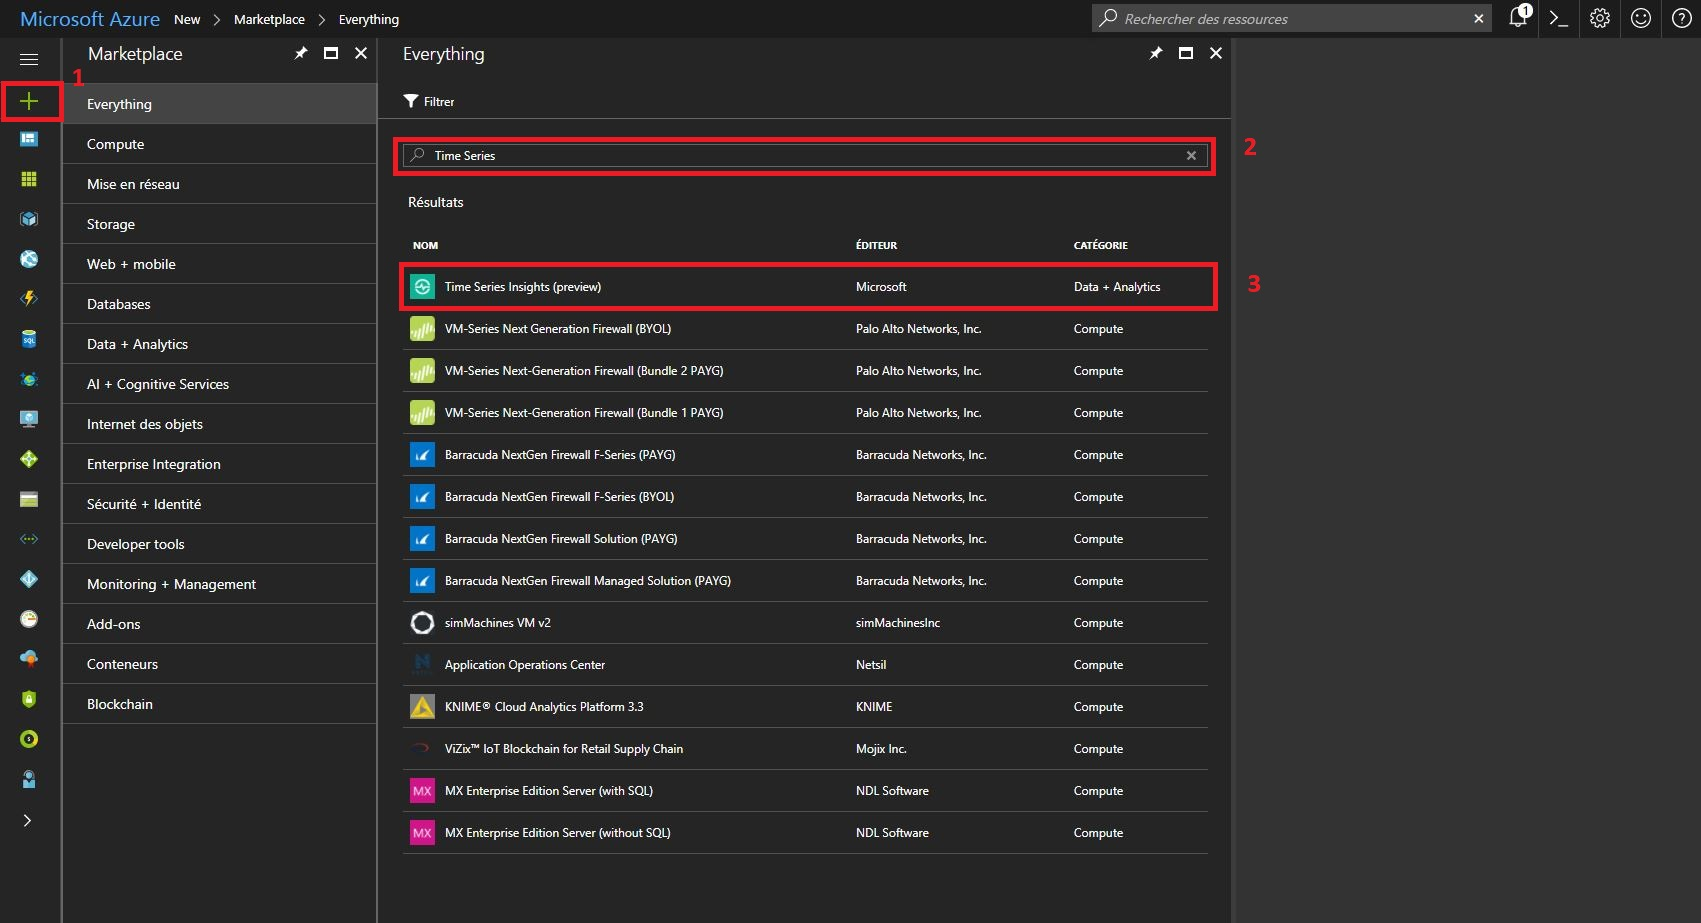
\includegraphics[width=.7\paperwidth]{images/azure_portal_1.jpg}}
\end{center}
	\caption{ \textit{Menu de recherche de ressources sur Azure}}
\end{figure}\\

	\item Cliquer alors sur \textit{Créer}.\\
Vous arrivez alors sur la fenêtre  suivante :\\

\begin{figure}[H]
\begin{center}
	\makebox[\textwidth]{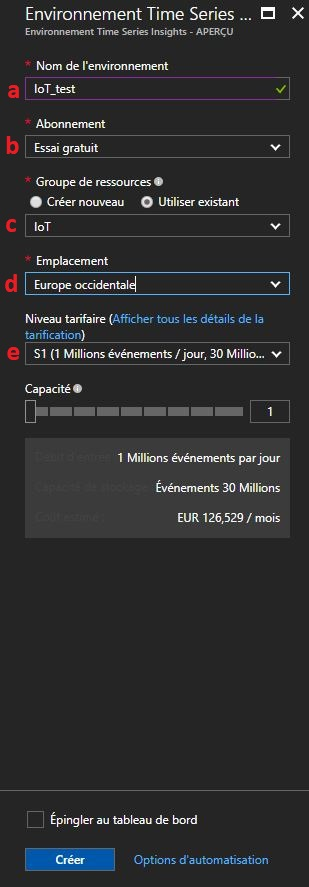
\includegraphics[width=.4\paperwidth]{images/azure_portal_2.jpg}}
\end{center}
	\caption{ \textit{Menu de recherche de ressources sur Azure}}
\end{figure}\\

\begin{enumerate}

	\item Il s'agit du nom que vous voulez donner à votre Portail. Ce nom apparaitra sur le Portail, donc préférez un nom qui vous indique les données qui vont y être envoyer.
	
	\item Choisissez votre abonnement \textit{azure}.
	
	\item Choisissez le groupe de ressources que nous avons créée tout à l'heure. Pour le dossier, il s'agissait du groupe \textit{"IoT"}.
	\item Sélectionner \textit{"Europe Occidentale"}. C'est le serveur sur lequel va être implanté le portail.
	
	\item Pour ce choix, cela dépendra de votre besoin. Sachez que ce choix détermine le tarif du portail. Pour information, la station envoie ses données environ toute les deux minutes. Il n'était pas possible de mettre un délai plus long auquel cas il y aurait des problème de déconnexion de la station. Partez du principe qu'une station envoie 1000 évènements par jour, cela vous donne une indication quant aux nombre de stations que vous pouvez implémenter sur le portail.
	\item Cliquer alors sur \textit{Créer}.
	
\end{enumerate} \\
\end{enumerate}

Voilà, votre portail est en cours de déploiement, nous allons maintenant devoir faire en sorte que cette instance écoute les valeurs que l'on envoie sur le Hub d'évènement.

\subsection{Ajout d'une source d'évènements dans le portail \textit{Time Series Insights}}

Maintenant que vous avez créer votre instance \textit{Time Series Insights}, cliquer dessus pour voir sa page principale affichée :\\

\begin{figure}[H]
\begin{center}
	\makebox[\textwidth]{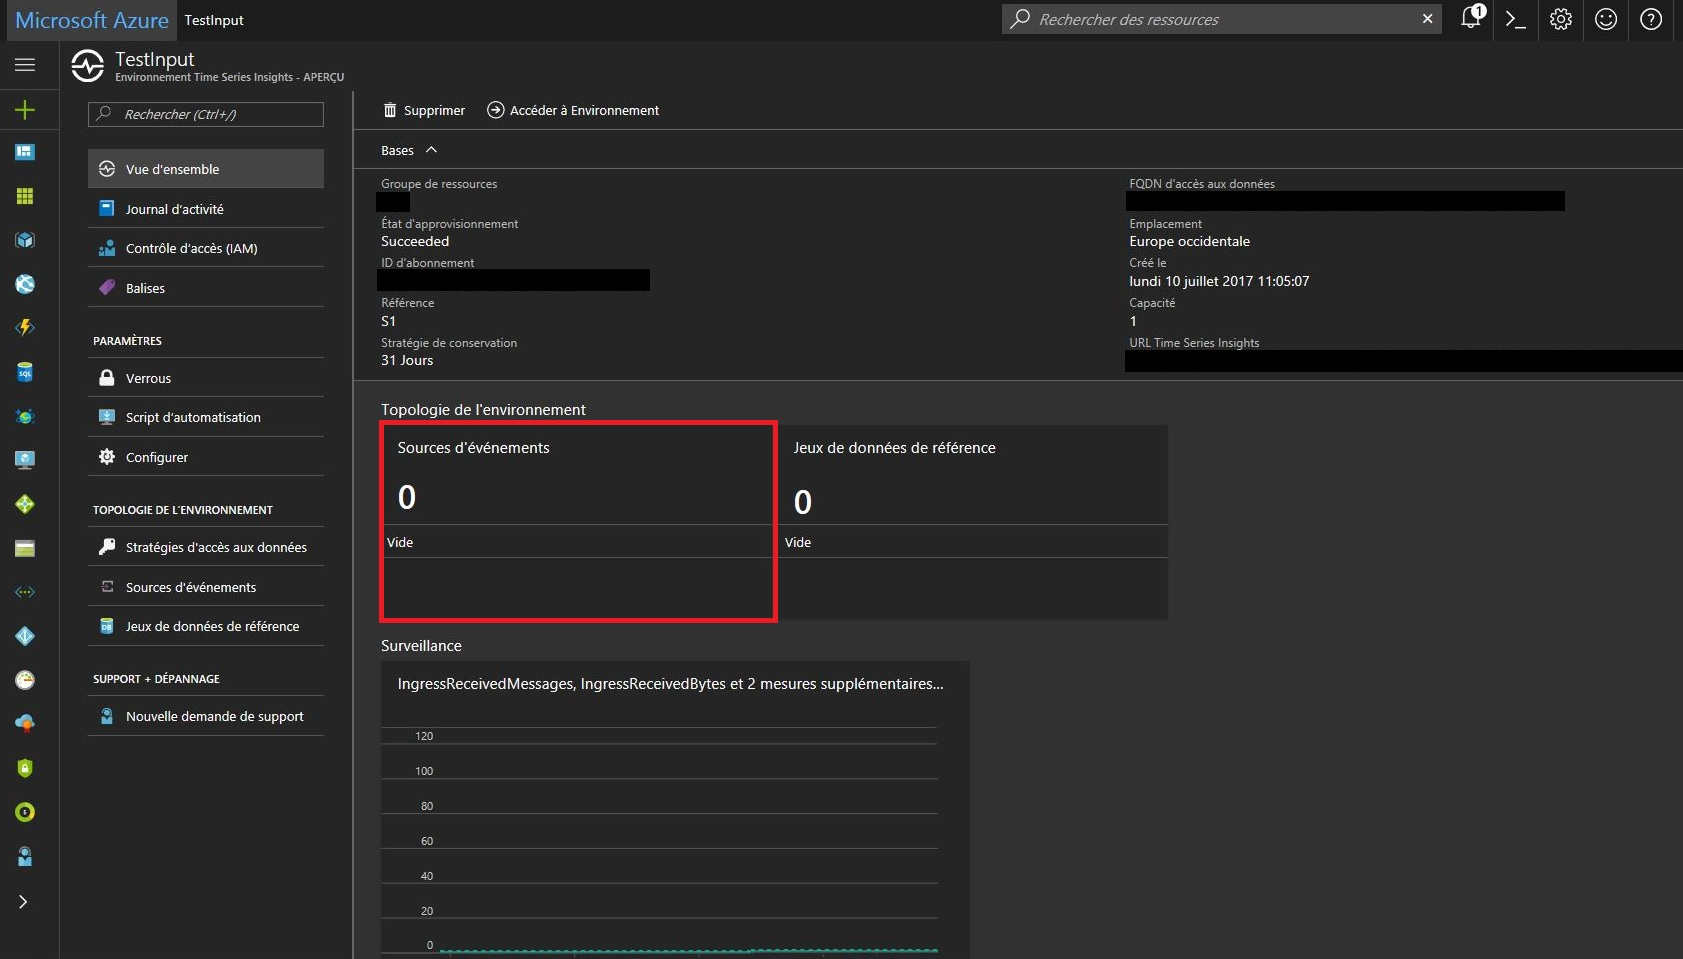
\includegraphics[width=.7\paperwidth]{images/azure_portal_3.jpg}}
\end{center}
	\caption{ \textit{Menu principal du \textit{Time Series Insights}}}
\end{figure}\\

\begin{enumerate}
	\item Cliquer sur la zone \textit{Sources d'évènements} puis sur \textit{Ajouter} en haut dans la fenêtre qui s'ouvrira.
	\item vous devriez alors voir apparaitre cette fenêtre : 
	\begin{figure}[H]
\begin{center}
	\makebox[\textwidth]{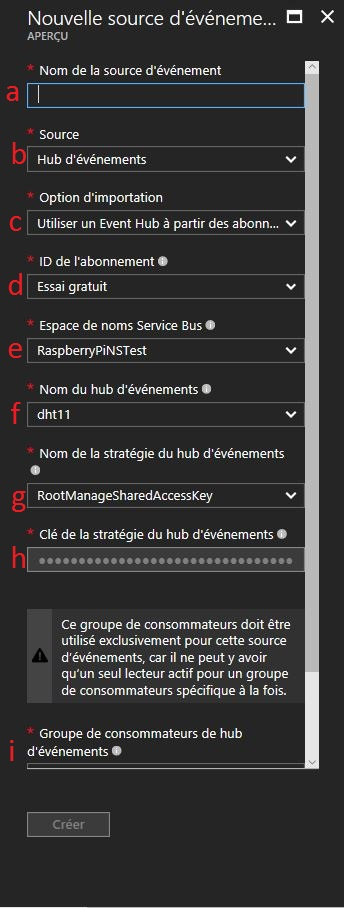
\includegraphics[width=.4\paperwidth]{images/azure_portal_4.jpg}}
\end{center}
	\caption{ \textit{Ajout d'une source d'évènements}}
\end{figure}\\
	\begin{enumerate}
	\item C'est le nom que vous voulez donner à votre source. Le choix est arbitraire.
	\item Choisir \textit{Hub d'évènements}.
	\item Choisi \textit{Utiliser un Event Hub à partir des abonn..}
	\item Ici, le champs dépend de votre abonnement.
	\item Pour les étapes qui vont suivre, il sera nécessaire de reprendre les champs indiqué lors de la section~\ref{CLI} page~\pageref{CLI}. Pour le premier, entrer le \textit{namespaceName}.
	\item Ici doit être indiqué \textit{l'evenHubName}.
	\item Le choix \textit{RootManageSharedAccessKey} devrait être proposé. Il s'agit probablement de votre \textit{SharedAccessKeyName}. Sinon, renseigner votre \textit{SharedAccessKeyName}
	\item Renseigner votre \textit{SharedAccessKey}
	\item Ici doit être entré votre \textit{consumerGroupName}.
	\item laisser ce dernier champs vide et cliquer sur \textit{Créer}.
	\end{enumerate}
\end{enumerate}\\

Vous avez donc ajouté le hub d'évènement comme source pour l'instance de \textit{Time Series Insights}. Il reste alors à éditer le code de la station pour indiquer le hub sur lequel envoyer les données.


\subsection{Configuration logiciel de la station pour \textit{Azure}}

Avant de vous montrer les modifications à réaliser dans le code, quelques informations concernant celui ci. Le code est écrit dans le langage \href{https://www.python.org/}{Python}. En plus d'avoir le mérite d'être considéré comme un des langages les plus haut niveau (ie. proche du langage de l'Homme et donc intuitif), il est particulièrement adapté pour l'utilisation de script automatisé comme vous allez le faire pour la station.\\

\textbf{ATTENTION : Avant de vous faire découvrir le code et de vous expliquer les lignes à modifier pour pouvoir envoyer vos données, une petite explication sur l'architecture d'un code Python. Il est impératif de respecter les indentations (espacement) du code. Si jamais vous rajouter ne serait-ce qu'un espace sur une ligne, cela peut avoir comme effet de faire planter l'intégralité de la station. Si cela ce produit, pour simplifier le problème, reportez vous à l'annexe N°1.}\\

Il reste cependant une étape avant de modifier le code. En effet, il est nécessaire d'installer la bibliothèque azure sur la \textit{RaspberryPi}. Pour cela, connectez vous en ssh dessus puis entrer la commande :\\

\begin{lstlisting}[style=MyBashStyle]
	sudo pip install azure-servicebus
\end{lstlisting}\\

Nous pouvons désormais regarder le code :\\ 
\newpage
\pythonexternal{../rpi/test_complet.py}\\

Maintenant que vous avez le code à disposition avec les lignes, vous allez pouvoir réaliser les changements de manière un peu plus lisible. Pour éditer le fichier, effectuer la commande :

\begin{lstlisting}[style=MyBashStyle]
	sudo nano /home/pi/DrancIoT/code/
\end{lstlisting}\\











	
	




